\documentclass[11pt]{article}

% ---------- packages ----------
\usepackage[utf8]{inputenc}
\usepackage[T1]{fontenc}
\usepackage{lmodern}
\usepackage[margin=1in]{geometry}
\usepackage{amsmath,amssymb}
\usepackage{booktabs}
\usepackage{array}
\usepackage{graphicx}
\usepackage{xcolor}
\usepackage{tikz}
\usetikzlibrary{arrows.meta,positioning}
\usepackage{caption}
\usepackage{enumitem}
\usepackage[hidelinks]{hyperref}
\usepackage{microtype}

\captionsetup{font=small,labelfont=bf}
\setlength{\parskip}{0.35em}
\setlength{\emergencystretch}{3em}
\newcommand{\code}[1]{\texttt{\small #1}}

% ---------- title ----------
\title{\bfseries LLM-Enhanced Process-Aware Knowledge Tracing\\
from Student Solution Steps for Concept Deficiency Prediction}
\author{Temesgen\\[2pt]
\normalsize University of Vienna}
\date{June 2026}

\begin{document}
\maketitle

\begin{abstract}
\noindent
Most knowledge tracing (KT) systems only predict whether a student will get the
next question right. The recent ConceptKT benchmark asks a harder and more useful
question: which of $55$ math concepts will a student be weak in on their next
problem? Trained KT models do this very poorly, and only large language models
(LLMs), used directly at prediction time, do reasonably well, but they are slow and
costly to run. This report tests a middle path. We run a small, low-cost Gemini model once on each
\emph{past} solution, offline, to pull out a few simple signals: the concepts the
student seems to have missed, the type of error, the faulty step, and a short
summary of what happened. A small LSTM then learns from these past-only signals to
predict the student's future weak concepts. On the official MathEDU/ConceptKT split
($3{,}644$ train and $404$ test interactions from $6$ students), averaged over five
random seeds, the LLM signals raise deficiency macro-F1 over $13$ categories from
$24.0\%$ (a correctness-only baseline) to $28.3\%$. That covers about $60\%$ of the
gap to a gold-feature ceiling of $31.1\%$, and both precision and recall improve. We
block label leakage with a runtime check that we test to make sure it actually fires,
and the full run repeats offline with the same numbers. The short answer to the
research question is yes: even with very little data, LLM signals taken from solution
steps help.
\end{abstract}

% =====================================================================
\section{Introduction}
% =====================================================================
Knowledge tracing tries to follow how a student's understanding changes over time and
to predict how they will do next. Classic methods look only at which questions were
asked, the skills involved, and whether each answer was right or wrong
\cite{piech2015dkt}. This works well for predicting the next answer, but it throws
away the student's actual working, which often says far more about what they
misunderstand than the final answer does \cite{huang2024remembering}.

Newer work has started to use the solution process itself, and to bring language
models in for their semantic and reasoning signals
\cite{lee2024lkt,park2025statuskt,ozyurt2024kcqrl}. The ConceptKT benchmark
\cite{kang2026conceptkt} pushes this further by changing the task. Instead of
predicting a single right or wrong bit, it asks which specific concepts a student is
currently weak in. This is useful, because it tells a teacher what to go back over,
but it is also hard. On ConceptKT the trained KT baselines are almost useless at it
(the best, OKT, gets $1.87\%$ macro-F1), and only a full LLM reaches about $17\%$.

We study the question from the proposal:
\begin{quote}\itshape
Can LLM-derived process signals from student solution steps improve concept
deficiency prediction compared with a correctness-only baseline?
\end{quote}

The key idea is to use the LLM as an offline analyzer, not as the predictor. It reads
each past solution once and writes down a few structured signals. A small trained
model then uses those signals to predict future weak concepts. This plays to each
part's strength: the LLM is good at reading one solution, and a tiny LSTM is a
sensible choice when there are only six students. The work has three parts. First, a
complete and repeatable pipeline (an offline Gemini analyzer with a disk cache, careful
sequence building, and a two-head LSTM). Second, a clean three-way comparison that
separates the value of the LLM signals from everything else and also measures how
much better a perfect analyzer could do. Third, an honest setup: leakage is blocked and
tested, the class imbalance is handled directly, results are averaged over five seeds,
and the whole thing reruns offline.

The headline is simple. The offline LLM signals add $4.3$ points of macro-F1@13 over
the baseline and close about $60\%$ of the gap to gold features. With six students and
$59$ positive test labels the exact decimals jump around, so the result to trust is
the order, A below B below C, rather than the precise values.

% =====================================================================
\section{Related Work}
% =====================================================================
Deep Knowledge Tracing brought neural sequence models to KT and set the standard way
of predicting performance from a history of interactions \cite{piech2015dkt}. Later
models refined the backbone but still read only correctness and skill ids. A separate
line argues that remembering a fact is not the same as applying it, and models the
solving process for the sake of interpretability \cite{huang2024remembering}. We share
that motivation but aim at the harder concept-deficiency output instead of correctness.

Text and language models have also been folded into KT. Using language-model
representations of question and concept text helps, especially for cold-start items
where there is little history \cite{lee2024lkt}. KCQRL shows that an LLM can label
knowledge concepts at the level of each solution step, and that the resulting
concept-aligned embeddings improve $15$ different KT models on two large datasets
\cite{ozyurt2024kcqrl}. That is the basis for two of our choices: getting concept and
process signals from an LLM, and turning the LLM's short summary into a fixed sentence
embedding.

The closest method is StatusKT, which runs a three-stage LLM pipeline to read
proficiency signals out of solving processes and feeds them into existing KT models,
improving both accuracy and interpretability over correctness-only KT
\cite{park2025statuskt}. We follow the same idea, an LLM that produces structured
signals for a trained KT model, but in a much smaller, low-resource form, and we
measure the signals against a gold-feature ceiling. The task, label set, and split all
come from ConceptKT \cite{kang2026conceptkt}, which is built on MathEDU, a set of real
student solutions with correctness labels, teacher error notes, and feedback
\cite{hsu2026mathedu}. ConceptKT runs its LLM end-to-end at prediction time; the
trained baselines it reports use only correctness. Our hybrid sits between those two.

% =====================================================================
\section{Data}
% =====================================================================
We use two public repositories from the NYCU NLP Lab that describe the same $4{,}048$
interactions from $6$ students, seen from two sides. MathEDU \cite{hsu2026mathedu} is
the process side: each record has a problem \code{id}, a \code{student\_id}, the final
answer, the worked solution in \LaTeX, a correctness label, and, when wrong, a teacher
note with an error type and a faulty equation. ConceptKT \cite{kang2026conceptkt} is
the label side: for every record it gives the gold \code{associated\_concepts} (what
the problem needs) and \code{missing\_concepts} (what the student failed to apply,
empty when correct), from a fixed list of $55$ concepts in $13$ categories. It also
ships the official $90/10$ split in time order ($3{,}644$ train and $404$ test).

We merge the two on the pair \code{(id, student\_id)}, which matches all
$4{,}048$ records with no gaps; \code{id} on its own is not unique because students
share MathQA problems. ConceptKT acts as the backbone of the merge, since it owns the
time order, the official split, and the gold labels, and MathEDU's process fields hang
off it. Two small things had to be handled so the split lines up exactly: two repeated
\code{(id, student\_id)} rows from a re-attempt, which we resolve by taking the later
copy for the test set, and MathEDU's eight raw error strings, which we fold into a
six-way set of error types. One point is easy to get wrong: the time order is the
position inside ConceptKT, grouped by student. The \code{id} is a problem number, not a
timestamp, so the data must never be sorted by it.

Table~\ref{tab:data} sums up the corpus, and three facts from it shaped the design.
The data is very lopsided: $75.3\%$ of answers are correct, and only $463$ records
($11.4\%$) carry a real deficiency target. The signal is also thin at test time, with
just $59$ positive concept labels spread across the $404$ test targets, which makes
macro-F1 noisy and is why we lean on imbalance-aware loss, threshold tuning, and a
coarser $13$-category view. Finally, MathEDU has no question text, so the analyzer works
from the solution alone. That does not touch the deficiency targets, which are gold.

\begin{table}[t]
\centering
\caption{MathEDU/ConceptKT corpus statistics.}
\label{tab:data}
\small
\begin{tabular}{@{}lr@{\hspace{2.2em}}lr@{}}
\toprule
\textbf{Quantity} & \textbf{Value} & \textbf{Quantity} & \textbf{Value}\\
\midrule
Interactions            & $4{,}048$ & Concepts / categories      & $55$ / $13$\\
Students                & $6$       & Correct answers            & $3{,}050$ ($75.3\%$)\\
Train / test (official) & $3{,}644$ / $404$ & Wrong answers      & $998$ ($24.7\%$)\\
Records with gold deficiency & $463$ ($11.4\%$) & Concept mistakes & $722$ ($17.8\%$)\\
Test positive concept labels & $59$  & Careless errors            & $276$ ($6.8\%$)\\
\bottomrule
\end{tabular}
\end{table}

% =====================================================================
\section{Method}
% =====================================================================
Figure~\ref{fig:pipeline} shows the flow. Each raw record goes through the LLM analyzer,
gets turned into numbers, is placed into a leakage-safe sequence, and is fed to a
two-head LSTM whose deficiency head is limited to the concepts the target question
actually needs.

\begin{figure}[t]
\centering
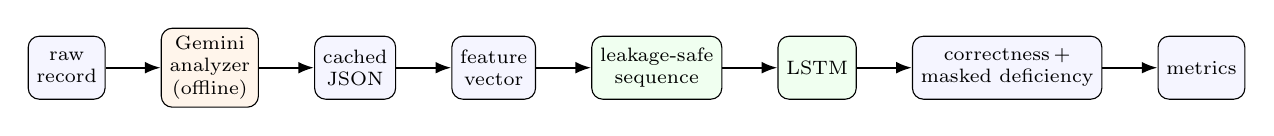
\begin{tikzpicture}[
  node distance=6mm and 7mm,
  box/.style={draw,rounded corners,align=center,inner sep=3pt,font=\scriptsize,
              minimum height=8mm,fill=blue!4},
  arr/.style={-{Latex[length=2mm]},thick}
]
\node[box] (raw) {raw\\record};
\node[box,right=of raw,fill=orange!8] (llm) {Gemini\\analyzer\\(offline)};
\node[box,right=of llm] (cache) {cached\\JSON};
\node[box,right=of cache] (feat) {feature\\vector};
\node[box,right=of feat,fill=green!6] (seq) {leakage-safe\\sequence};
\node[box,right=of seq,fill=green!6] (dkt) {LSTM};
\node[box,right=of dkt] (heads) {correctness\,+\\masked deficiency};
\node[box,right=of heads] (met) {metrics};
\draw[arr] (raw)--(llm); \draw[arr] (llm)--(cache); \draw[arr] (cache)--(feat);
\draw[arr] (feat)--(seq); \draw[arr] (seq)--(dkt); \draw[arr] (dkt)--(heads);
\draw[arr] (heads)--(met);
\end{tikzpicture}
\caption{The full data flow. The LLM is called once per past interaction and its
output is saved. Everything after it is a small model that runs the same way every
time.}
\label{fig:pipeline}
\end{figure}

\subsection{The offline LLM analyzer}
For each interaction the analyzer makes one call to Gemini (model
\code{gemini-3.1-flash-lite}, taken from an environment variable so the model can be
swapped without touching code). The prompt asks it to describe what already happened
in the solution and to return a fixed JSON object: the associated concepts, the
missing concepts, a six-way error type, the faulty step, a note on partial
understanding, and a one or two sentence summary. A JSON schema forces the shape of
the answer. A few choices keep this part cheap and reliable. The temperature is set to
zero, so the same input always gives the same output. Every result is saved to disk
under a key built from the prompt and model, so re-running the pipeline makes no API
calls at all and identical solutions share a file. The first extraction made
$3{,}882$ live calls with zero failures and produced $3{,}962$ cached results that
cover all $4{,}048$ interactions, for well under \$5. We picked a small, low-cost model
on purpose, to keep the whole extraction cheap; a larger state-of-the-art LLM would most
likely read the solutions more accurately and give cleaner signals, a point we return to
in the discussion. A system message keeps the model
in line: it must pick concepts only from the fixed $55$, and for a correct answer it
must leave the missing list empty and the error type as \code{none}. A small
cleanup step afterwards drops any made-up concept and re-checks those rules, so a
sloppy answer cannot corrupt the labels. Failures are split on purpose: a malformed
answer is retried once and then stored as an empty placeholder, while a real API or
key error is retried once and then raised, never cached, so a bad key cannot poison the
cache.

\subsection{Turning signals into features}
Each interaction becomes the components in Table~\ref{tab:features}. The error type is
passed as a small id and learned as an $8$-dimensional embedding inside the model,
since a small category like this is better learned than hand-set. The summary is
turned into a vector by a frozen \code{all-MiniLM-L6-v2} sentence encoder
\cite{reimers2019sbert}; with six students there is no data to train an encoder, so we
just use it as a fixed way to read meaning out of the text, much as KCQRL does
\cite{ozyurt2024kcqrl}.

\begin{table}[t]
\centering
\caption{Per-interaction feature parts and which arms use them. The associated
concepts are known when the question is shown, so they also serve as the output mask.}
\label{tab:features}
\small
\begin{tabular}{@{}llcl@{}}
\toprule
\textbf{Component} & \textbf{Dim} & \textbf{Used by} & \textbf{Source}\\
\midrule
\code{assoc\_multihot}        & $55$  & A, B, C & gold associated concepts (and mask)\\
\code{correct}                & $1$   & A, B, C & grading\\
\code{llm\_missing\_multihot} & $55$  & B       & analyzer's missing concepts\\
\code{llm\_error\_type}       & emb.  & B       & analyzer's error type\\
\code{summary\_embed}         & $384$ & B       & frozen encoding of the summary\\
\code{gold\_missing\_multihot}& $55$  & C (and target) & gold missing concepts\\
\code{gold\_error\_type}      & emb.  & C       & gold (normalized) error type\\
\bottomrule
\end{tabular}
\end{table}

\subsection{A leakage-safe sequence model}
We build one sequence per student in time order. At step $i$ the model sees the
features of interaction $i$ and predicts interaction $i\!+\!1$. Because the prediction
for a target comes from the LSTM state after reading only the steps before it, a
target's own features never reach the model that predicts it. The backbone is a plain
single-layer LSTM (hidden size $64$, dropout $0.4$) with two heads on the next-step
state. The correctness head is one output trained with cross-entropy. The deficiency
head has $55$ outputs, but since a missing concept is always one of the associated
ones, we push the outputs for the rest down to a very large negative value before the
loss and the prediction. This drops about $53$ of $55$ obvious negatives per example
and lets the model focus on the real candidates. Those remaining outputs are trained
with a focal version of cross-entropy \cite{lin2017focal}, which lowers the weight of
the many easy negatives. The model is kept small on purpose, because with six students
anything bigger just memorizes.

\subsection{The three arms}
All three arms use the same LSTM and the same training code, and each one is trained
separately from scratch. The only thing that changes is the per-step input, so any
difference in the results comes from the features, not the model.
\begin{itemize}[leftmargin=1.4em,itemsep=2pt,topsep=2pt]
\item \textbf{Arm A (baseline).} Associated concepts plus the correct/wrong bit. This is
the correctness-only model: what you can predict from a pass/fail record with no LLM.
\item \textbf{Arm B (process-aware).} Arm A plus the analyzer's signals, that is, its
missing concepts, the summary vector, and the learned error embedding. This is the
system we are testing.
\item \textbf{Arm C (gold ceiling).} Arm A plus the \emph{gold} missing concepts and
gold error type taken from the human labels, used only for past steps. These are perfect
signals, so arm C is an upper bound on what any analyzer could reach.
\end{itemize}
The two comparisons that matter are B minus A, the value of the LLM signals over plain
correctness, and C minus B, how much a sharper analyzer could still add. A useful check
falls out of the design: arms A and C never touch the LLM, so they come out the same
whether we run on synthetic features or the real Gemini ones. Only arm B moves, which is
exactly what we want.

\subsection{Blocking leakage on purpose}
\label{sec:leakage}
The rule is that nothing about a target may be seen before predicting it, and the
analyzer must never see the target's own solution. We make this part of the structure
rather than a habit. The analyzer only ever gets one finished interaction at a time. The
model is causal by construction. The gold missing concepts are the target, and they
are used as an input only by arm C and only for past steps. On top of that, a runtime
check runs on every sequence and confirms that each target comes strictly after every
input used to predict it. To be sure the check works, a small negative test feeds it a
sequence with leakage on purpose and confirms the check fires. Using the associated
concepts as an input and a mask is not leakage, since they are known the moment the
question appears.

% =====================================================================
\section{Experimental Setup}
% =====================================================================
We use the official split ($3{,}644$ train and $404$ test). For early stopping we hold
out the last $10\%$ of each student's training history as validation, still before any
test target. Each arm and seed is trained with Adam (learning rate $10^{-3}$) for up to
$60$ epochs, stopping early on validation loss with a patience of $8$. The feature
store is built once and shared across arms and seeds, and we report mean and standard
deviation over five seeds.

The deficiency head needs one extra step. It is so imbalanced that a fixed $0.5$ cutoff
predicts all-negative and macro-F1 falls to zero, which would hide any difference
between arms. So after training we try a small grid of thresholds and keep the one that
gives the best macro-F1 on validation, then apply it once to the test set. The cutoff
is picked on validation and never on test. We score correctness with accuracy and AUC,
and deficiency with macro precision, recall, and F1 at both the $55$-concept level and
the steadier $13$-category level. With five fixed seeds, the official split, and a warm
cache, training makes no API calls and reproduces the saved metrics exactly. A set of
$45$ unit tests, none of which need the API, guards the taxonomy, the feature layout,
the leakage check, the caching and cleanup, the metrics, and the model shapes.

% =====================================================================
\section{Results}
% =====================================================================
Before trusting the analyzer on all $4{,}048$ records, we checked it against the gold
teacher notes on $20$ wrong answers. It matched the gold error type on $15$ of $20$
($75\%$), with many exact faulty-step matches. The misses sit on the fuzzy line between
a calculation error and a wrong-concept error, which is hard even for people, so we
went ahead.

Table~\ref{tab:main} has the main numbers, and the order is the same on every
deficiency metric: A below B below C.

\begin{table}[t]
\centering
\caption{Deficiency prediction on the official test set, mean and standard deviation
over five seeds. Correctness accuracy is flat because that head is swamped by the
$75\%$ rate of correct answers. Deficiency is where the process signals matter.}
\label{tab:main}
\small
\begin{tabular}{@{}lcccccc@{}}
\toprule
\textbf{Arm} & \textbf{Acc.} & \textbf{AUC} &
\textbf{F1@55} & \textbf{F1@13} & \textbf{P@13} & \textbf{R@13}\\
\midrule
A: correctness-only       & $71.78$ & $0.59$ & $10.28$ & $24.04$ & $19.29$ & $39.49$\\
\textbf{B: process-aware} & $71.78$ & $0.59$ & $\mathbf{12.24}$ & $\mathbf{28.31}$ & $25.16$ & $47.24$\\
C: gold ceiling           & $71.78$ & $0.59$ & $13.36$ & $31.10$ & $28.78$ & $45.60$\\
\midrule
\multicolumn{2}{@{}l}{std on F1@13} & & & \multicolumn{3}{l}{A: $\pm4.18$\quad B: $\pm4.73$\quad C: $\pm1.46$}\\
\bottomrule
\end{tabular}
\end{table}

Three things stand out. The LLM signals help: arm B beats arm A by $4.3$ points of
macro-F1@13 ($24.04$ to $28.31$) and $2.0$ points at the concept level ($10.28$ to
$12.24$), and both precision and recall go up, so it is not just a threshold trick. The
signals also recover most of the gap to gold: the full room from A to C is $7.1$
points, and arm B reaches $28.31$, about $60\%$ of the way, leaving $2.8$ points that a
sharper analyzer could still add. And correctness stays flat at $71.78\%$ across all
arms, because that head is dominated by the base rate of correct answers. Correctness
is simply not where these signals pay off; deficiency is, which is what ConceptKT found
too \cite{kang2026conceptkt}.

Table~\ref{tab:erroranalysis} breaks the B minus A difference down by category. The
signals help most on multi-step and word-problem topics, Sequences and Series ($+0.35$),
Physics ($+0.12$), and Statistics and Probability ($+0.10$), where reading the working
helps tell concept mistakes apart in a way that raw correctness cannot. A few
categories slip a little (Polynomials $-0.07$, Finance $-0.03$, Geometry $-0.02$), most
likely because the extra features add noise where correctness was already a fine guide.
Across the $13$ categories, six improve, four stay the same, and three drop.

\begin{table}[t]
\centering
\caption{Per-category deficiency F1 (mean over seeds), arm B minus arm A. A positive
value means the LLM signals helped that category. Categories with no test positives are
left out.}
\label{tab:erroranalysis}
\small
\begin{tabular}{@{}lccc@{}}
\toprule
\textbf{Category} & \textbf{A} & \textbf{B} & \textbf{Change}\\
\midrule
Sequences and Series        & $0.114$ & $0.460$ & $+0.346$\\
Physics                     & $0.114$ & $0.237$ & $+0.123$\\
Statistics and Probability  & $0.000$ & $0.096$ & $+0.096$\\
Ratio and Proportion        & $0.000$ & $0.053$ & $+0.053$\\
Set Theory                  & $0.133$ & $0.178$ & $+0.044$\\
Prime Numbers               & $0.391$ & $0.397$ & $+0.006$\\
Geometry                    & $0.533$ & $0.515$ & $-0.019$\\
Finance                     & $0.481$ & $0.454$ & $-0.027$\\
Polynomials                 & $0.500$ & $0.433$ & $-0.067$\\
\bottomrule
\end{tabular}
\end{table}

For context, Table~\ref{tab:context} shows the numbers ConceptKT reports
\cite{kang2026conceptkt}. The trained KT models predict correctness fairly well
($63$ to $69\%$) but are close to useless on deficiency (OKT gets $1.87\%$), and only a
full LLM reaches about $17\%$. This is context, not a fair race. We use the same split
and gold labels, but our setup is different (a small model on past-only offline
features against their end-to-end LLM), and our $13$-category F1 is a coarser score than
their $55$-concept macro-F1. The comparison we control cleanly is the A, B, C contrast
in Table~\ref{tab:main}.

\begin{table}[t]
\centering
\caption{ConceptKT baselines \cite{kang2026conceptkt}, for context only, not directly
comparable to Table~\ref{tab:main}.}
\label{tab:context}
\small
\begin{tabular}{@{}lcc@{}}
\toprule
\textbf{Method} & \textbf{Correctness acc.} & \textbf{Deficiency macro-F1}\\
\midrule
DKT                       & $64.80$ & n/a\\
DKVMN                     & $63.10$ & n/a\\
GKT                       & $63.20$ & n/a\\
SAKT                      & $66.46$ & n/a\\
OKT                       & $69.25$ & $1.87$\\
Best LLM (DeepSeek-R1)    & $71.02$ & $17.40$\\
\bottomrule
\end{tabular}
\end{table}

% =====================================================================
\section{Discussion}
% =====================================================================
The answer to the research question is a careful yes. Offline LLM signals from solution
steps do improve concept deficiency prediction over correctness alone, by $4.3$ points
of macro-F1@13, with gains in both precision and recall and a steady A, B, C order
across seeds and both levels of detail. The gain comes from features that are read once,
offline, from each past solution, and the model that uses them is small and cheap to
run. That is exactly the role the proposal set out to test: the LLM as an analyzer of the
process, not as the predictor.

Arm C earns its place as a yardstick rather than just a baseline. By covering about
$60\%$ of the A to C room, arm B shows that the offline analyzer already captures most of
the signal in these features, and the $2.8$ points left over put a number on what a
better analyzer could add. Part of that leftover gap is likely down to the model we
chose: we ran a small, low-cost LLM to keep the extraction cheap, and a bigger
state-of-the-art model would probably read the solutions more accurately and recover more
of those $2.8$ points. The $75\%$ agreement between the analyzer and the gold error
types fits that leftover gap. It is worth being plain about the noise. With six students
and $59$ positive test labels, the per-seed F1@13 moves by several points, so the order
is the real result, not the decimals. Arm C's much tighter spread ($\pm1.46$) is itself
a sign that cleaner features both raise and steady the score.

% =====================================================================
\section{Limitations and Future Work}
% =====================================================================
The dataset is tiny, six students and $59$ positive test labels, so the numbers are
noisy and the conclusions point in a direction rather than pin down a value. MathEDU has
no question text, so the analyzer works from the solution only, though the targets are
gold and so unaffected. We use one prompt and a single small, low-cost LLM, chosen to keep costs down, with no
sensitivity study, and the backbone is a plain LSTM rather than a state-of-the-art KT
model.

A few next steps would help, roughly in order of value. Swapping the LSTM for a stronger
backbone such as SAKT or DKVMN through pyKT \cite{liu2022pykt}, while keeping
the same features, is the obvious first move. Replacing the plain concatenation of
features with a learned gate would let the model turn down noisy analyzer signals when
they are not helping. A leave-one-student-out test would be a fairer check of
generalization than the time split given only six students. A prompt-sensitivity study
would show whether the offline-feature idea is stable, which is the whole point. Joining
the real question text from MathQA and re-reading would test whether more context helps
the analyzer. Finally, a per-concept threshold instead of one global cutoff could squeeze
out a bit more.

% =====================================================================
\section{Conclusion}
% =====================================================================
We built a small, repeatable hybrid for concept deficiency prediction. A Gemini model
reads each past solution once, offline, and writes down a few structured signals, and a
small leakage-safe LSTM learns from those past-only signals to predict future weak
concepts. On the official MathEDU/ConceptKT split, the LLM signals raise deficiency
macro-F1@13 from $24.0\%$ to $28.3\%$ over a correctness-only baseline and cover about
$60\%$ of the gap to a gold-feature ceiling of $31.1\%$, with both precision and recall
improving. The result comes with a tested leakage guarantee, direct handling of the
class imbalance, five-seed reporting, and full offline reproducibility. With very little
data, turning student solution steps into simple structured signals with an offline LLM
is a practical way to make diagnostic KT better.

% =====================================================================
\begin{thebibliography}{99}
\setlength{\itemsep}{2pt}

\bibitem{piech2015dkt}
C.~Piech, J.~Bassen, J.~Huang, S.~Ganguli, M.~Sahami, L.~J.~Guibas, and
J.~Sohl-Dickstein, ``Deep Knowledge Tracing,'' in \emph{Advances in Neural
Information Processing Systems (NeurIPS)}, 2015.

\bibitem{huang2024remembering}
T.~Huang, X.~Ou, H.~Yang, Z.~Long, and C.~Xing, ``Remembering is Not Applying:
Interpretable Knowledge Tracing for Problem-Solving Processes,'' in \emph{Proc.\ 32nd
ACM Int.\ Conf.\ on Multimedia (MM)}, 2024, doi:10.1145/3664647.3681049.

\bibitem{lee2024lkt}
U.~Lee, J.~Bae, D.~Kim, S.~Lee, J.~Park, T.~Ahn, G.~Lee, D.~Stratton, and H.~Kim,
``Language Model Can Do Knowledge Tracing: Simple but Effective Method to Integrate
Language Model and Knowledge Tracing Task,'' \emph{arXiv preprint arXiv:2406.02893},
2024.

\bibitem{hsu2026mathedu}
W.-L.~Hsu, Y.-C.~Tang, and A.-Z.~Yen, ``MathEDU: Feedback Generation on
Problem-Solving Processes for Mathematical Learning Support,'' in \emph{Proc.\ 19th
Conf.\ of the European Chapter of the Association for Computational Linguistics
(EACL)}, 2026.

\bibitem{kang2026conceptkt}
Y.-C.~Kang, Y.-C.~Tang, and A.-Z.~Yen, ``ConceptKT: A Benchmark for Concept-Level
Deficiency Prediction in Knowledge Tracing,'' \emph{arXiv preprint arXiv:2603.24073},
2026.

\bibitem{park2025statuskt}
J.~Park, S.~Kang, J.~Park, J.~Kim, J.~Shin, S.~Park, and Y.~Yu, ``Tracing
Mathematical Proficiency Through Problem-Solving Processes,'' \emph{arXiv preprint
arXiv:2512.00311}, 2025.

\bibitem{ozyurt2024kcqrl}
Y.~Ozyurt, S.~Feuerriegel, and M.~Sachan, ``Automated Knowledge Concept Annotation
and Question Representation Learning for Knowledge Tracing,'' \emph{arXiv preprint
arXiv:2410.01727}, 2024.

\bibitem{reimers2019sbert}
N.~Reimers and I.~Gurevych, ``Sentence-BERT: Sentence Embeddings using Siamese
BERT-Networks,'' in \emph{Proc.\ EMNLP-IJCNLP}, 2019.

\bibitem{lin2017focal}
T.-Y.~Lin, P.~Goyal, R.~Girshick, K.~He, and P.~Doll\'ar, ``Focal Loss for Dense
Object Detection,'' in \emph{Proc.\ IEEE Int.\ Conf.\ on Computer Vision (ICCV)},
2017.

\bibitem{liu2022pykt}
Z.~Liu, Q.~Liu, J.~Chen, S.~Huang, B.~Gao, W.~Luo, and J.~Weng, ``pyKT: A Python
Library to Benchmark Deep Learning based Knowledge Tracing Models,'' in \emph{NeurIPS
Datasets and Benchmarks Track}, 2022.

\end{thebibliography}

\end{document}
